% This document must be compiled with LuaLaTeX
\documentclass[12pt,article]{memoir}

\usepackage[letterpaper, portrait, margin=1in]{geometry}	% Standard page setup
\usepackage[USenglish]{babel}								% English typsetting conventions
\usepackage{fancyhdr}										% Headers and footers
\usepackage{graphicx}										% Additional graphics options
\usepackage{xcolor}											% Better colors
\usepackage{xpatch}											% Better macro patches
\usepackage{hyperref}										% Hyperlinks
\usepackage{fontspec}										% Custom fonts
\usepackage{tikz}											% Graphics creation
\usepackage{float}											% Figure positioning
\usepackage{tabu}											% Better tables
\usepackage[style=ieee, backend=biber]{biblatex}			% Bibliography
\usepackage[font={small,it}]{caption}						% Italic captions
\usepackage{textcomp}
\usepackage{hhline}
\setsansfont{NeueHaasUnicaPro}
\usetikzlibrary{calc}
\usepackage[yyyymmdd]{datetime} % change date format to yyyy/mm/dd to fit ISO8601

\renewcommand{\familydefault}{\sfdefault} % set font
\renewcommand{\dateseparator}{--} % change date-seperators to - to fit ISO8601

\renewcommand\contentsname{Table of Contents}

\chapterstyle{section}
\renewcommand*{\chapnumfont}{\normalfont\HUGE\bfseries\sffamily}
\renewcommand*{\chaptitlefont}{\normalfont\HUGE\bfseries\sffamily}

\makeatletter 
% define macro for itemcode
\newcommand\itemcode[1]{\renewcommand\@itemcode{#1}}
\newcommand\@itemcode{}

% define macro for rev number
\newcommand\revnumber[1]{\renewcommand\@revnumber{#1}}
\newcommand\@revnumber{}
\makeatother

\definecolor{orbitOrange}{RGB}{250,62,0} % the ORBiT orange

\setlrmarginsandblock{2.5cm}{2.5cm}{*}
\setulmarginsandblock{2.5cm}{*}{1}
\checkandfixthelayout 

\setlength{\beforechapskip}{0cm} % reduce chapter spacing

\hypersetup{
    colorlinks,
    citecolor=black,
    filecolor=black,
    linkcolor=black,
    urlcolor=black
}

% Background swoosh
\newcommand\OrbitBackground[1]{% For a logo drawn with TikZ
	\begin{tikzpicture}[remember picture,overlay] % draw background
	\coordinate (bl) at (current page.south west);
	\coordinate (r) at (current page.east);
	\coordinate (A) at ($(bl)+(0,3cm)$);
	\coordinate (B) at ($(r)+(0,-2cm)$);
	\coordinate (C) at (current page.south east);
	\coordinate (ctrlNode) at ($(current page.south) + (0cm,1cm)$);
	\coordinate (ctrlNode2) at ($(current page.south east) + (-1cm,1cm)$);
	\fill[orbitOrange, fill opacity={#1}]
	(A) .. controls (ctrlNode) and (ctrlNode2) .. (B) -- (C) -- (bl);
	\node [white] at ($(C) + (-3cm,1cm)$) {2015-\the\year \ ORBiT@SU};
	\end{tikzpicture}
}

%**********************************************************************
% Document titles etc. defined here: (replace [] as well)
\title{TELXX-YYWW\_CE CONRAD}
\author{Cem Eden}
\itemcode{DS00001}
\revnumber{A04}
\date{\today}
% End of document titles etc.
%**********************************************************************

% set header style
\makeatletter
\pagestyle{fancy}
{
	\fancyheadoffset{0cm}

	\lhead{\@title \ - \@itemcode}
	\rhead{Page: \thepage }
	%\chead{\leftmark} % section name
}
\makeatother

\cfoot{\OrbitBackground{0.2}}

\begin{document}
	
\OrbitBackground{1}

\makeatletter

\includegraphics[width=\textwidth]{../Templates/logo.jpg}\\[4ex]
\begin{center}
	\bfseries \fontsize{50}{50}\selectfont  \@title \\[2ex]
	\LARGE  \@itemcode
\end{center}
\vfill
\begin{flushright}
	\LARGE Rev: \@revnumber\\
	\large \@author\\
	\large \@date\\[18ex]
\end{flushright}
\makeatother
\thispagestyle{empty}
\newpage

\tableofcontents*
\thispagestyle{fancy}
\newpage

\tableofcontents*
\clearpage

%**********************************************************************
% Everything after this is the main document. Edit below this line.

\chapter{Introduction}
\section{Quick Description}
The TELXX-YYWW\_CE (Conrad) board is the main telemetry board intended to be used in medium sized rockets or similarly sized aviation equipment. Its main function is to provide radio communications, GPS positioning as well as basic atmospheric data gathering.\par

\section{Main features}
The Conrad board includes an attachment position to provide a secure connection for an XTend radio module (XTPB-DMD-001) to provide radio communications. To allow for maximum range, the module is powered with 5V, with a 3V voltage level shifter IC to allow for seamless communication with the main flight computer.\par
The board itself contains a GPS module (RMX-GNS-TM) to provide accurate positioning data for flight tracking purposes. To counter long locking GPS period on initial powerup, the board allows for a selectable power supply for the internal clock of the GPS module. The selection can be made using a soldered jumper, located in close proximity to the GPS module.\par
For increased Positioning accuracy, the Conrad board includes an accelerometer (BMX055).\par
For basic atmospheric data gathering the Conrad board contains a combined temperature, pressure and humidity IC (BME280). This module is intended to provide basic atmospheric information, but due to its hard positioning will be used for interior monitoring of the vehicle.\par
Due to limitations of the intended flight computer, communication busses are limited. To counteract this, the accelerometer IC and atmospheric probe share a common SPI bus. Selecting an IC to communicate with is realized by GPIO pins (More information in \autoref{chap:Communication}).\par

\newpage

\chapter{Electrical Specifications}
\section{Absolute Maximum Ratings}
\begin{tabularx}{\textwidth}{|l|X|c|c|}
	\hline
	Symbol & Parameter & Value  & Unit\\\hhline{|=|=|=|=|}
	V\textsubscript{cc} & Power supply & 5.5 & V\\\hline
	V\textsubscript{bat} & GPS backup battery & 4.3 & V\\\hline
	V\textsubscript{in} & Signal input voltages & 3.6 & V\\\hline
	T\textsubscript{op} & Operating temperature range & -40 to +85 & \textdegree{}C\\\hline
\end{tabularx}
\section{Electrical Characteristics}
\begin{tabularx}{\textwidth}{|l|X|X|c|c|c|c|}
	\hline
	Symbol & Parameter & Testing Conditions & Min. &Typ. & Max. &Unit\\\hhline{|=|=|=|=|=|=|=|}
	V\textsubscript{cc} & Power supply & Operative condition & 4.75 & 5 & 5.5 & V\\ \hline
	I\textsubscript{cc} & Peak V\textsubscript{cc} current & Peak & & & 2000 & mA\\ \hline
	V\textsubscript{IO} & GPIO voltages & Operative condition \textsubscript{bat} & 1.2 & 3.3 & 3.6 & V \\ \hline
	V\textsubscript{bat} & GPS backup battery & JMP1 = V\textsubscript{bat} & 2.0 & & 4.3 & V \\ \hline
	T\textsubscript{op} & Operating temperature & Operative condition  & -40 & +25 & +80 & \textdegree{}C \\ \hline
\end{tabularx}

\clearpage

\section{Pin Layout}
\begin{center}
	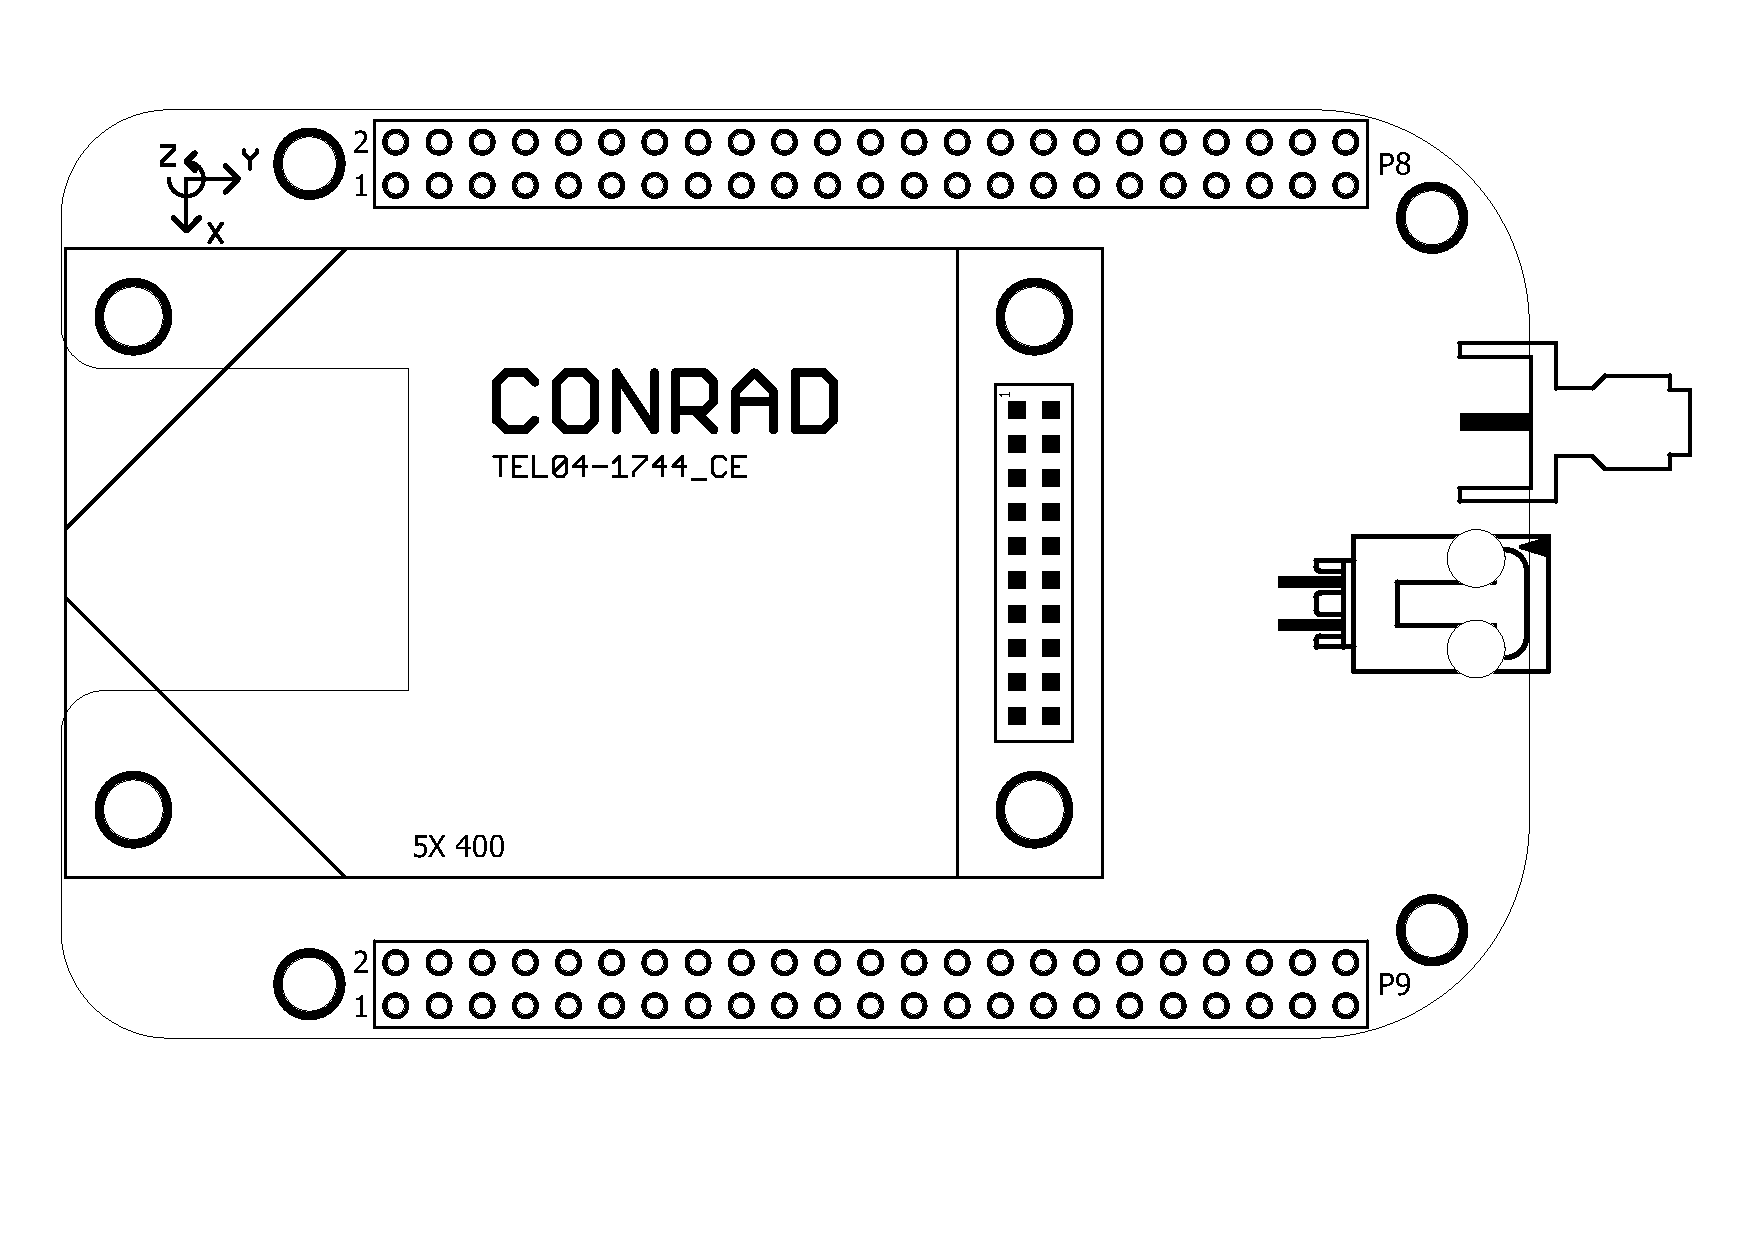
\includegraphics[width=5.5in]{DS00001_pinouts.pdf}
\end{center}\par

\begin{tabularx}{\textwidth}{|l|m{4.7cm}|X|}
	\hline
	Pin name & Pin number(s) & Functionality\\\hhline{|=|=|=|}
	V\textsubscript{cc} & P9.5, P9.6& Power supply \\\hline
	GND & P8.1, P8.2, P9.1, P9.2, P9.43, P9.44, P9.45, P9.46 & Circuit ground\\\hhline{|=|=|=|}
	
	UART1\_TX & P9.13 & Radio module serial\\\cline{1-2}
	UART1\_RX & P9.11 & \\\cline{1-2}
	UART1\_CTSN & P8.32 & \\\cline{1-2}
	UART1\_RTSN & P8.33 & \\\hhline{|=|=|=|}
	
	UART2\_TX & P8.38 & GPS module serial\\\cline{1-2}
	UART2\_RX & P8.37 & \\\hhline{|=|=|=|}
	
	SPI\_CLK & P9.22 & SPI Bus\\\cline{1-2}
	SPI\_CS & P9.17 & \\\cline{1-2}
	SPI\_SDI & P9.18 & \\\cline{1-2}
	SPI\_SDO & P9.21 & \\\hline
	
	A0 & P8.26 & SPI chip select addressing \\\cline{1-2}
	A1 & P8.27 & \\\cline{1-2}
	A2 & P8.28 & \\\hline
	
\end{tabularx}

\newpage

\chapter{Communication}
\label{chap:Communication}

\section{RMX-GNS-TM (GPS)}
Communications with the GPS is realized using a serial interface. By default, the data rate is set to 9,600bps with 8 data bits, 1 start bit, 1 stop bit and no parity. The GPS uses the serial pins UART2.

\section{XTPB-DMD-001 (Radio)}
Communications with the radio interface is realized through a serial interface. The data rate is defined by the settings in the XTPB-DMD-001 module, and will have to be accounted for when establishing initial communications. After a factory reset of the radio module, the baud rate will be set to be 9,600bps with 1 start bit, 1 stop bit and no parity. The radio module uses the serial pins UART1.

\section{BME280 (Atmospheric probe)}
Communications with the BME280 is realized using the SPI bus. However, the chip is multiplexed with other SPI devices with the use a chip select. In order to select the BME280, the address pins A[2:0] have to be set to 000. The BMX280 uses the SPI pins for the SPI bus.

\section{BMX055 (Accelerometer/Gyroscope/Magnetometer)}
Communications with the BMX055 is realized using the SPI bus. However, The BMX055 is multiplexed with other SPI devices, as well as its own functionalities. The BMX055 uses the SPI pins for the SPI bus. The BMX055 uses three addresses on A[2:0] of 1 through 3 inclusive. The addresses of each functionality is given in the table below:
\begin{table}[h]
\centering
\begin{tabular}{|c|c|}
	\hline
	Function & Address A[2:0]\\ \hline
	Accelerometer & 001\\ \hline
	Gyroscope & 010\\ \hline
	Magnetometer & 011\\ \hline
\end{tabular}
\end{table}

\newpage

\chapter{Usage}
\section{Device Tree Overlays}
The Conrad board is designed to be used as a cape for a Beaglebone Black. To set the correct modes for the used pins, a device tree overlay(dto) has to be loaded prior to using some of the features provided by the Conrad board. Information on where to find and how to use the device tree overlay can be found in the "software and Setup" manual.

\section{Software}
To utilize the ICs on the Conrad board, software is required. Previously written software may be used, for which information can be found in the "Software and Setup" manual. Custom software can also be written to handle tasks for which previous software may be insufficient.

\newpage

\chapter{Product Code}
Each version of the Conrad board is uniquely identified by an alphanumeric product code. This code is comprised by a version number, date of last design alteration and initials of the original designer.\par
The Code is defined as shown below:

\begin{table}[h]
\centering
\definecolor{shadecolor1}{RGB}{210,210,210}
\definecolor{shadecolor2}{RGB}{170,170,170}
\definecolor{shadecolor3}{RGB}{210,210,210}
\definecolor{shadecolor4}{RGB}{170,170,170}
\begin{tabular}{|c|}
	\hline
	\huge \\
	\huge TEL\colorbox{shadecolor1}{XX}-\colorbox{shadecolor2}{YY}\colorbox{shadecolor3}{WW}\_\colorbox{shadecolor4}{AA} \\
	
	\colorbox{shadecolor1}{XX} - Version | \colorbox{shadecolor2}{YY} - Year | \colorbox{shadecolor3}{WW} - Week | \colorbox{shadecolor4}{AA} - Original Designer\\
	
	\hline
\end{tabular}
\end{table}
\noindent
As of writing, the most recent version of the Conrad board is TEL04-1744\_CE.

% End of document.
%**********************************************************************
\end{document}